\section{Background}
In this section, we briefly introduce the types of scientific application from aspect of task dependencies, then we introduce the workflow system that support those using scenarios and explain the shortage of current workflow system.

\subsection{Types of Scientific Application and Workflow System}
Considering the scientific application in \cite{makeflowexample}, the execution of tasks in workflow could be represented as DAG, every node represent the execution of the task and every edge represent the sequence of the execution between tasks. For workflow in \cite{makeflowexample}, the abstraction of DAG could be acquired before the application running, then workflow will schedule and execute the task according to this DAG blueprint. There are some workflow framework such as \cite{albrecht2012makeflow,wilde2011swift} was designed to support these kind of dependencies fixed application. The intermediate file was used to control the execution of the typical dependency pattern\cite{bharathi2008characterization}.

There are other types applications without fixed and explicit task dependency pattern before the task running, the task triggering depends on the content of the data instead of the input/output data files in those cases. For example, in simulation-analyzing-visualization workflow, large amount of simulation data will be generated in short time, some simulation will also running several days, there are some redundant data in the output of the data but only some of them are useful data. If we only want to visualise the data  with average value larger than specific threshhold, the picture will be plotted only when data satisfy our predefined  condition. There are several strategies for workflow system to address this issue, one is post processing which will load all the simulation data into disk and then processing the data in separate tasks. But this solution only useful for small scale simulation, the increasing data, size and limited storage and bandwidth make high fidelity post-processing impractical\cite{ayachit2015paraview}. In situ workflow is the latest trend to solve this issue\cite{dreher2017situ}. There are several intermediate component to leverage the in-situ workflow\cite{docan2012dataspaces,ayachit2015paraview}  there are works exploring how to decompose original algorithm into in-situ method such as\cite{bennett2012combining} some works are exploring the properties of workflow at exascale\cite{dreher2017situ} but  few works focusing on how workflow support different type of in-situ tasks involving flexible dependencies relationship. 

\subsection{Types of Dependencies between Workflow Tasks}
One critical distinguish between the traditional workflow(without in-situ task) and the in-situ workflow is the construction of task dependencies. For traditional workflow such as \cite{albrecht2012makeflow}, the dependencies is determined by input and output files between tasks, for example, if the output file of task A is the input of the task B there is dependency between taskA and taskB namely taskB needed to be started after taskA finish.  In situ workflow, the dependency will be in fine granularity and flexible way.  For example, task B will start after one loop iteration of taskA finish, or taskB needed to be started when the output of taskA satisfy specific condition. Dedicated communication libraries needed to be used to send message between different tasks to  synchronise the execution of the task namely to decide when the task is supposed to be started. No matter for the traditional task or in situ tasks, the task dependency pattern could be divided into three main types \cite{albrecht2012makeflow,bharathi2008characterization} which are shown in Figure 1. 
\begin{figure*} 
\centering
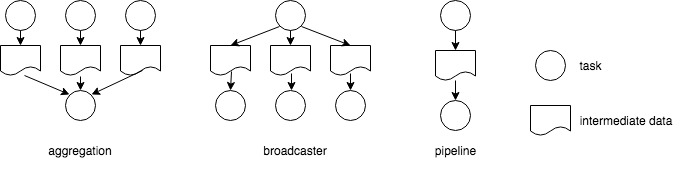
\includegraphics[width=.8\linewidth]{./figure/taskpattern.jpg}
\caption{typical workflow pattern}
 \label{fg:state}
\end{figure*} 

For traditional workflow, the intermediate data are files on the disk and the work queue\cite{albrecht2012makeflow} could be used to control the execution of tasks,  for in situ workflow, the intermediate data is event message generated by in-situ tasks and the task dispatching mechanism will be discussed in implementation.

\subsection{Pub-Sub paradigm and event driven workflow pattern}

If we treat the event message as a special intermediate data used to synchronise the task execution, Pub-Sub paradigm \cite{eugster2003many} could satisfy the requirements to run fine granularity task dependency by  messaging communication in distributed way, but there are few scientific workflow system combining the the task dependency and event driving programming together. Some works such as \cite{jin2012scalable} use this mechanism to leverage the in situ workflow, but they only support specific underlying library and the types of task dependency pattern is also limited. A canonical pub-sub mechanism works in three steps , assume there are two component namely subscriber $S$ and publisher $P$.(1) $S$ will subscribe one or more interested events into the pub-sub broker (2) $P$ will push events into the pub-sub broker (3)  pub-sub broker will notify $S$ if pushed event mach the subscribed event. There exists a dependency between publish and subscriber in this paradigm. If we use this programming model to compose workflow, the task could be a publisher or subscriber at in the workflow, there will be less restriction on task because any type of tasks could generate the event used to construct the dependency , the task can be in-situ part of the task or jobs running by sbatch system flexibly according to different using scenarios. By this task composing model,  This kind of event driven workflow should support the task paradigm in Figure 2:
\begin{figure*} 
\centering
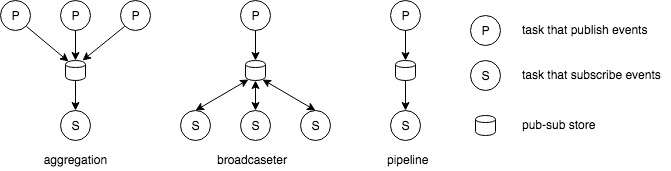
\includegraphics[width=.8\linewidth]{./figure/edtaskpattern.jpg}
\caption{typical event driven workflow pattern}
 \label{fg:state}
\end{figure*} 

The broadcaster and pipeline pattern are supported by pub-sub-notify mechanism naively but there is no support for aggregation pattern. For typical pub-sub mechanism, is subscriber subscribe multiple event such as eventA, eventB eventC, and publishing of those three event will notify the subscriber and triggering execution of task, however, in workflow aggregation scenario, the specific subscribed runtime is supposed to be triggered when all eventA , eventB and eventC are published and satisfied. We will discuss the details of pub-sub event store and relevant runtime client to support all of those pattern in implementation part. 
